%    Template for seminar reports
% Seminar Current Topics in Computer Vision and Machine Learning
% Summer Semester 2015
% Computer Vision Group, Visual Computing Institute, RWTH Aachen

\documentclass[twoside,a4paper,article]{combine}


% =========================================================================
\usepackage[utf8]{inputenc}
\usepackage[ngerman]{babel}
\usepackage{a4}
\usepackage{fancyhdr}   
%\usepackage{german}    % Uncomment this iff you're writing the report in German
\usepackage{makeidx}
\usepackage{color}
\usepackage{t1enc}		% german letters in the "\hyphenation" - command
\usepackage{latexsym}	% math symbols
\usepackage{amssymb}    % AMS symbol fonts for LaTeX.

\usepackage{graphicx}
\usepackage{pslatex}
\usepackage{ifthen}

\usepackage[T1]{fontenc}
\usepackage{pslatex}

\usepackage{psfrag}
\usepackage{subfigure}
\usepackage{url}

% =========================================================================

\setlength{\oddsidemargin}{3.6pt}
\setlength{\evensidemargin}{22.6pt}
\setlength{\textwidth}{426.8pt}
\setlength{\textheight}{654.4pt}
\setlength{\headsep}{18pt}
\setlength{\headheight}{15pt}
\setlength{\topmargin}{-41.7pt}
\setlength{\topskip}{10pt}
\setlength{\footskip}{42pt}

\setlength{\parindent}{0pt}

% =========================================================================

\graphicspath{
	{img/}
}

%%%
% We want also subsubsections to be enumerated
%%%
\setcounter{secnumdepth}{3}
\setcounter{tocdepth}{3}

\makeglossary
%\makeindex

% =========================================================================
\begin{document}

% Template for seminar reports
% Seminar Current Topics in Computer Vision and Machine Learning

\begin{titlepage}


\begin{center}
\ 
\vspace{3.5cm}


\textsf
{
Fakultät für Mathematik, Informatik und Naturwissenschaften\\
Lehr- und Forschungsgebiet Informatik VIII\\
Computer Vision\\
Prof. Dr. Bastian Leibe
}

\rule{\linewidth}{1pt}

\vspace{1.75cm}
\LARGE
\textbf{Seminar Report}

\vspace{1.7cm}
\huge
Combining 3D Shape, Color, and Motion for Robust Anytime Tracking

\vspace{3.0cm}
\Large
Frederik Zwilling\\
\large
Matriculation Number: 304314

\vspace{0.5cm}
June 2015

\vspace{1.05cm}
\rule{\linewidth}{1pt}

\vspace{0.5cm}
\textsf{\textbf{
\normalsize
\begin{tabular}{ll}
Advisor:  & Aljoša Ošep\\
\end{tabular}
}}
\end{center}

\end{titlepage}


\begin{abstract}
  \textcolor{red}{Abstract}
\end{abstract}

\tableofcontents
\newpage
% =========================================================================

\section{Introduction}
Robust and precise position and velocity estimation is an important
part of object tracking. It is an essential part in the collision
avaidance of an autonomous car, for example. This report presents a
method by Held, Levinson, Thrun, and Savarese to solve this part of
the tracking problem by combining the 3D shape, color and motion of
the tracked object~\cite{paper}. The method uses a probabilistic
measurement model in form of a Dynamic Bayesian Network. The state
space of position and velocity for each tracked object is represented
in a special dynamic histogram, called \textit{annealed dynamic
  histogram}. This histogram dynamically increases its resolution in
the important areas and considers the local resolution in the
measurement model. By expanding the measurement model with color the
method results can be further improved. This is shown by the authors
by evaluating in a static environment where only the reference system
is moving and in a dynamic environment where the compactness of the
models build with the tracking results is used as evaluation criteria. 


\subsection{Motivation}
Robotic applications are about to change many domains from the ground
up. Especially autonomous systems could take over dangerous,
exhausting and unpopular tasks and allow humans to do more satisfying
tasks instead. Additionally, autonomous systems can be more efficient
and scalable than solving the tasks by hand. Some progressive domains
with autonomous robots are flying drones, which can map
areas~\cite{auto-drones} or deliver
packages~\cite{auto-delivery-drones}, autonomous cars, which take care
of driving~\cite{auto-cars}, logistic robots, which store and grab
goods in warehouses~\cite{kiva}, and domestic service robots, which
can support old people and clean at home~\cite{athome}. All these
domains have in common that the robots have to track objects in their
environment, mostly for avoiding collisions, in the case of domestic
service robot also to follow people for example. Often the reliability
and precision of the tracking are limiting factors. An autonomous car,
for example, can only drive fast if it is absolutely sure that it
tracks all objects in the sorounding correctly and none of these
objects could cause a collision.  This report mainly focuses on the
domain of autonomous cars. Here, the autonomous system takes care of
the time consuming driving task on the one hand and could help to
reduce the amount of traffic deaths ($25,938$ in $2013$ in the
EU~\cite{traffic-deaths}) on the other hand. In this domain it is
especially important to estimate the speed of various nearby objects
robustly and in real time. Figure~\ref{fig:objects} shows the three
main classes of objects that have to be tracked, cars, bicycles, and
pedestrians, in challenging situations. The method proposed in this
report solves this task and performs better than previous approaches
in the car domain.
\begin{figure}
  \label{fig:objects}
  \subfigure[Cars on a highway]{%
    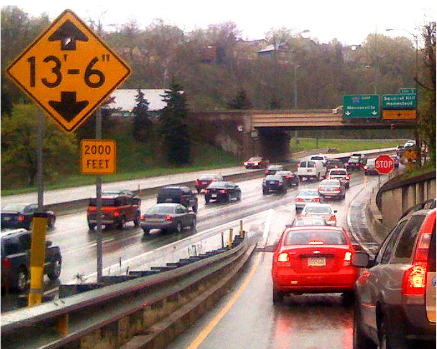
\includegraphics[height=.3\linewidth]{highway}
  }
  \subfigure[A cyclist]{%
    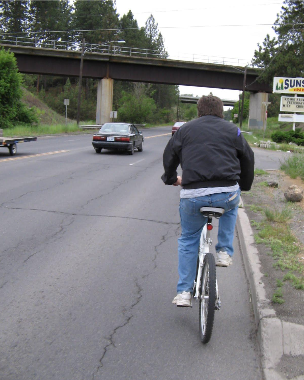
\includegraphics[height=.3\linewidth]{bicycle}
  }
  \subfigure[A pedestrian]{%
    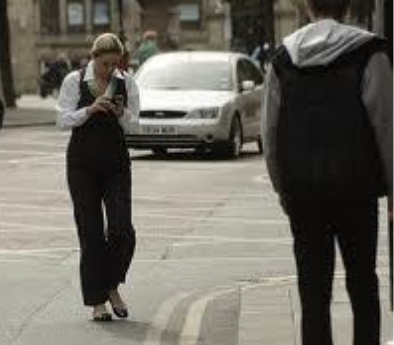
\includegraphics[height=.3\linewidth]{pedestrian}
  }
  
  \caption{Various objects that have to be tracked in challenging
    situations~\cite{held-website}}
\end{figure}


\subsection{Tracking}
Object tracking is the complex task to identify objects and their
movement over time. It can be seperated into the following parts. The
first step segments the sensor data for time $t$, called
\textit{frame}, into detected objects. This can be done for example by
seperating foreground and background and find connected components in
the foreground. In this step it is benificial to use that
the most important objects to find are cars, bicycles and
pedestrians~\cite{segmentation}. The second step is to associate
detected object in the successive frames $t$ and $t+1$. One method to
find these matchings is to compute descriptors, such as the HOG
descriptor, for the objects and find nearest neighbors in the
descriptor space~\cite{arbitrary-object-recognition}. The third step
is the position and velocity estimation of the tracked object. That is
the part of tracking this report is about.

The data that is used for tracking in this report is generated by a
dense laser sensor that measures the distance to sourounding objects
with multiple rotating laser beams. Such a sensor and the data
generated by it is shown in Figure~\ref{fig:lidar}. Additionally, the
sensor provides a camera image similar to a panorama.
\begin{figure}
  \label{fig:lidar}
  \center
  \subfigure[]{%
    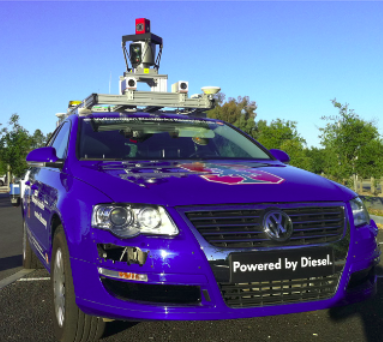
\includegraphics[height=.35\linewidth]{lidar}
  }
  \subfigure[]{%
    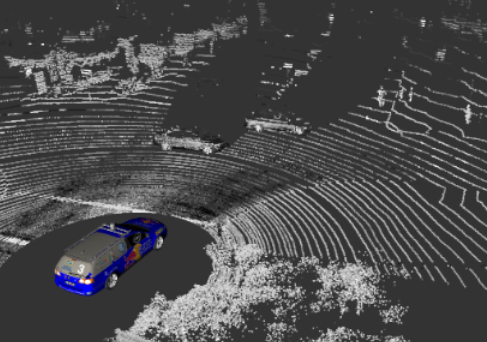
\includegraphics[height=.35\linewidth]{lidar-data}
  }
  
  \caption{A Velodyne LIDAR sensor mounted on a car (a) and a
    visualizaiton of the point cloud generated by it
    (b)~\cite{arbitrary-object-recognition}}
\end{figure}

\subsection{Velocity and Pose Estimation}
% +++++++++++++++++++++++++
\section{Related Work}
\subsection{Trajectory Classification}
\subsection{Grid-Based Methods}
\subsection{Alternative Sensors}

% +++++++++++++++++++++++++
\section{Method}
\subsection{Probabilistic Model}
\subsection{Annealed Dynamic Histograms}
\subsection{Adding Color}

% +++++++++++++++++++++++++
\section{Evaluation}
\subsection{Relative Reference Frame}
\subsection{Model Crispness}

% +++++++++++++++++++++++++
\section{Conclusion}


% =========================================================================
\bibliographystyle{alpha}
\bibliography{seminar_report}

% =========================================================================

\end{document}
